\documentclass[11pt]{article}

\usepackage[margin=1in]{geometry}
\usepackage{times}
\usepackage{setspace}
\usepackage{graphicx}
\usepackage{amsmath}
\usepackage{amssymb}
\usepackage[hidelinks]{hyperref}
\usepackage{booktabs}
\usepackage{float}
\usepackage{array}
\usepackage{algorithm}
\usepackage{algpseudocode}
\usepackage{xcolor}
\usepackage{listings}

\onehalfspacing

\lstset{
  basicstyle=\ttfamily\small,
  breaklines=true,
  frame=single,
  backgroundcolor=\color{gray!8},
  columns=fullflexible
}

\title{\textbf{SentinelAgent: Risk-Adaptive Policy Enforcement for Tool-Using LLM Agents Under Indirect Prompt Injection}}
\author{Pranav Kumar Kaliaperumal\\University of Colorado Denver\\\texttt{pranavkumar.kaliaperumal@ucdenver.edu}}
\date{May 13, 2026}

\begin{document}
\maketitle

\begin{abstract}
Tool-using large language model (LLM) agents can retrieve private documents, call external services, write state, and send messages. Those capabilities make prompt injection more than a text classification problem. A malicious instruction becomes more dangerous when the agent can connect it to tools with private-read, external-write, database-write, or code-execution permissions. Our project, SentinelAgent, studies this setting through a machine-learning-assisted policy enforcement framework for tool-using agents exposed to indirect prompt injection, data exfiltration, and unsafe tool-use attacks. The core system combines a supervised prompt-injection classifier with a permission-aware policy engine that models attack source, attack goal, target boundary, tool permissions, risk level, and enforcement action. We evaluate the artifact offline on a generated benchmark with 500 adversarial and 300 benign scenarios, plus a 440-case adaptive attack suite. In the benchmark split, full SentinelAgent reduces attack success from 100.0\% with no defense to 14.4\%, with 0.0\% measured secret leakage, but it also produces a 40.0\% false-positive rate under the current conservative policy. The injection classifier reaches 94.0\% accuracy, 100.0\% precision, 88.0\% recall, and 0.940 AUROC on its held-out test split. On adaptive attacks, our results still show residual failures, including 16.4\% attack success and 50.9\% secret-leakage rate under the local simulator. We also include a small Gemini-backed validation using \texttt{gemini-2.5-flash-lite}; it records 0.0\% attack success over 12 stratified tasks, but we treat that LLM API run as an additional integration check rather than the main evaluation. These results support a bounded claim: ML-assisted, permission-aware middleware can reduce measured attack success under a controlled threat model, but the present prototype is not yet a production-grade guarantee.
\end{abstract}

\section{Introduction}

LLM agents increasingly sit between users and tools. They search knowledge bases, summarize documents, fetch web pages, analyze data, update records, and draft messages. This design changes the security problem. In a chat-only system, prompt injection can produce a bad answer. In a tool-using agent, the same injected text may steer the planner toward a private document search, a database update, an outbound message, or a code-execution path.

SentinelAgent starts from a simple observation: prompt-injection risk depends on the tools available to the agent. A malicious string embedded in a retrieved document is not equally risky in every setting. If the only available tool is a calculator, the string has little operational leverage. If the agent can read private documents and send messages, the same string may become a practical exfiltration path. This paper reframes SentinelAgent as a risk-adaptive policy layer for that permission-sensitive setting.

Our system is middleware rather than a replacement for model alignment. It treats model-facing content as untrusted, records the source of suspicious instructions, applies the learned injection detector, scores exfiltration signals, looks up tool permissions, and chooses an enforcement action. The policy can allow, monitor, redact, require confirmation, block a tool call, block a response, or terminate a session. We preserve a deterministic mode for reproducibility and add an optional LLM-backed agent mode for model-in-the-loop validation.

This work makes four contributions:
\begin{itemize}
  \item A formal taxonomy covering attack source, attack goal, target boundary, tool permission, risk level, and enforcement action.
  \item A portable supervised injection classifier, permission registry, and risk-adaptive policy engine for tool-using agents under indirect prompt injection and exfiltration pressure.
  \item A reproducible benchmark generator, adaptive attack suite, evaluation runner, classifier evaluation path, statistical analysis script, and artifact documentation.
  \item An empirical report based on generated local results, a small Gemini-backed validation, ablations, and limitations where the prototype still fails.
\end{itemize}

\section{Background and Motivation}

Prompt injection exploits the fact that LLMs process instructions and data in the same natural-language channel. Direct prompt injection appears in a user request. Indirect prompt injection appears in content the agent later retrieves or observes, such as a document, web page, email, or tool output. Prior work has shown that indirect prompt injection can compromise real LLM-integrated applications when untrusted content is placed into the model context \cite{greshake2023not}. Recent benchmark and formalization work makes the same point from another angle: agent security depends on where instructions enter the system, which tools are available, and how the evaluation counts policy violations \cite{liu2024formalizing,zhan2024injecagent,debenedetti2024agentdojo}.

Tool-using agents sharpen this risk. The question is no longer only whether text is malicious. The relevant question is whether malicious text can influence a boundary with meaningful permissions. An instruction hidden in a retrieved policy document may be harmless if it only reaches a summarizer. It becomes more serious if the same agent can search private files, update a database, or send content outside the organization.

SentinelAgent therefore uses permission-aware enforcement. It borrows the security intuition behind least privilege and defense in depth: sensitive actions should be mediated by controls outside the model, and each boundary should have an audit record. The implementation does not assume that prompt wording alone can solve prompt injection.

\section{Threat Model}

The adversary controls text that enters the agent. This includes user prompts, retrieved documents, web content, tool outputs, memory entries, and multi-turn context. The adversary may try to override instructions, leak secrets, misuse tools, bypass policy, persist malicious instructions, corrupt data, or escalate privileges.

The adversary does not directly compromise the Python process, host operating system, source code, dependency chain, model weights, API gateway, or authentication system. The evaluation is a content-layer study. It asks whether middleware decisions reduce policy violations when malicious text reaches the agent, not whether SentinelAgent can withstand infrastructure compromise.

\begin{table}[H]
\centering
\caption{Threat taxonomy used by SentinelAgent}
\label{tab:taxonomy}
\begin{tabular}{p{0.22\textwidth}p{0.68\textwidth}}
\toprule
\textbf{Dimension} & \textbf{Values} \\
\midrule
Attack source & user prompt, retrieved document, web content, tool output, memory, multi-turn context \\
Attack goal & instruction override, secret exfiltration, unsafe tool use, policy bypass, persistence, data corruption, privilege escalation \\
Target boundary & input screening, retrieval context, agent planner, tool call, tool output, final response \\
Risk level & low, medium, high, critical \\
Enforcement action & allow, allow with monitoring, allow with redaction, require user confirmation, block tool call, block response, block session \\
\bottomrule
\end{tabular}
\end{table}

\section{Attack and Permission Taxonomy}

The taxonomy is implemented in \path{backend/sentinel_agent/research/taxonomy.py}. Each benchmark scenario contains a scenario identifier, source, goal, target boundary, tool context, required permissions, expected enforcement action, difficulty, payload, benign-equivalent task, and metadata. This makes the evaluation inspectable: a failure can be traced to a boundary and permission profile rather than buried in one aggregate security score.

\begin{table}[H]
\centering
\caption{Default tool permission registry}
\label{tab:tool_permissions}
\begin{tabular}{lll}
\toprule
\textbf{Tool} & \textbf{Permissions} & \textbf{Default risk} \\
\midrule
\texttt{calculator} & \texttt{read\_none} & low \\
\texttt{web\_fetcher} & \texttt{read\_public, network\_read} & medium \\
\texttt{document\_search} & \texttt{read\_private} & high \\
\texttt{message\_sender} & \texttt{write\_external, send\_message} & critical \\
\texttt{data\_analysis} & \texttt{read\_private} & high \\
\texttt{database\_read} & \texttt{database\_read, read\_private} & high \\
\texttt{database\_write} & \texttt{database\_write, write\_private} & critical \\
\texttt{shell\_executor} & \texttt{execute\_code} & critical \\
\bottomrule
\end{tabular}
\end{table}

The registry intentionally separates public reads, private reads, writes, external sends, database mutation, memory access, and code execution. These distinctions matter in policy. A suspicious retrieved document may be admitted with monitoring when the downstream tool only reads private context, but the same suspicion should block a code-execution tool or require explicit confirmation before an external message is sent.

\section{SentinelAgent Design}

SentinelAgent evaluates five enforcement boundaries:
\begin{itemize}
  \item \textbf{Input screening:} direct user prompts are checked before planning.
  \item \textbf{Retrieval-context screening:} retrieved documents and web content are treated as untrusted evidence.
  \item \textbf{Tool-call enforcement:} proposed tool names and arguments are evaluated against permissions, detector scores, canary presence, and domain policy.
  \item \textbf{Tool-output screening:} returned tool text is checked before it can influence subsequent reasoning.
  \item \textbf{Final-response control:} the response is checked for canary tokens, sensitive data, and exfiltration patterns before release.
\end{itemize}

The design is deterministic by default. SentinelAgent's main detector is a supervised n-gram Naive Bayes classifier trained from bundled benign and adversarial examples. The classifier produces a malicious-probability score, confidence value, and top evidence features. The policy engine then combines that ML score with exfiltration score, permissions, attack source, optional attack goal, sensitive-data presence, canary-token presence, domain allowlist result, and user-confirmation requirements. The engine returns a structured decision with the action, risk level, confidence, reasons, triggered rules, permissions considered, optional sanitized content, and a confirmation flag.

\subsection{Machine-Learning Detector}

The machine-learning component is the center of our project. It gives SentinelAgent a portable learned signal that can run inside the reproducible artifact without downloading model weights. The current classifier uses token and phrase features, n-gram evidence, and smoothed class likelihoods to separate benign operational requests from instruction override, exfiltration, and unsafe tool-use attempts. This choice is intentionally modest. A small classifier is easier to inspect, easier to ship with the artifact, and stable across machines, while still letting us measure how a learned detector changes enforcement behavior.

The detector is not the policy by itself. Its score feeds the policy engine, where tool permissions decide how severe the same text should be. A suspicious instruction attached to a calculator should not trigger the same response as suspicious text attached to an external message sender or shell executor. That interaction between ML scoring and permission-aware enforcement is the main research claim we test.

\begin{algorithm}[H]
\caption{Risk-adaptive tool-call decision}
\begin{algorithmic}[1]
\Require tool name $t$, arguments $a$, detector scores, source, optional goal
\State $P \gets$ permissions registered for $t$
\State $r \gets$ maximum risk implied by $P$, injection score, and exfiltration score
\If{arguments contain a canary token and $P$ includes outbound permission}
  \State \Return block tool call
\EndIf
\If{$t$ has network permission and destination is off allowlist}
  \State \Return block tool call
\EndIf
\If{$P$ includes code execution and injection is detected}
  \State \Return block tool call
\EndIf
\If{$P$ includes external send and injection is detected}
  \State \Return block or require user confirmation according to detector confidence
\EndIf
\If{$P$ includes private read and suspicious context is present}
  \State \Return allow with monitoring
\EndIf
\State \Return allow
\end{algorithmic}
\end{algorithm}

\begin{algorithm}[H]
\caption{Retrieval-context screening}
\begin{algorithmic}[1]
\Require retrieved chunk $c$, source label, injection score
\If{$c$ contains obvious instruction override language}
  \State mark triggered rule \texttt{injection\_detected}
\EndIf
\If{risk is high and downstream permissions include side effects}
  \State block or quarantine the chunk
\ElsIf{risk is suspicious}
  \State admit the chunk with monitoring metadata
\Else
  \State admit the chunk
\EndIf
\end{algorithmic}
\end{algorithm}

\begin{algorithm}[H]
\caption{Output exfiltration control}
\begin{algorithmic}[1]
\Require final response $y$
\If{$y$ contains a canary token}
  \State \Return block response
\EndIf
\If{$y$ contains sensitive-pattern disclosure}
  \State redact or block according to risk
\EndIf
\If{$y$ appears encoded or obfuscated with secret markers}
  \State raise risk and require stronger enforcement
\EndIf
\State \Return allow
\end{algorithmic}
\end{algorithm}

\section{Implementation}

The backend implementation is written in Python and organized under \path{backend/sentinel_agent}. The new research-facing modules are:
\begin{itemize}
  \item \path{research/taxonomy.py}: enums and dataclasses for scenario and decision records.
  \item \path{security/permissions.py}: tool-permission registry and risk classification helpers.
  \item \path{security/ml_injection_model.py}: portable supervised injection classifier used by the runtime detector.
  \item \path{security/policy_engine.py}: deterministic risk-adaptive policy engine.
  \item \path{agent/llm_agent.py}: optional mock, Gemini, or OpenAI-compatible LLM agent wrapper.
  \item \path{benchmark/generator.py}: benchmark and classifier dataset generator.
  \item \path{benchmark/adaptive_attacks.py}: adaptive transformation suite.
\end{itemize}

The LLM-backed mode is optional. It reads \texttt{SENTINEL\_AGENT\_MODE}, \texttt{SENTINEL\_LLM\_PROVIDER}, \texttt{SENTINEL\_LLM\_MODEL}, and provider keys such as \texttt{GEMINI\_API\_KEY}, \texttt{GEMINI\_API\_KEY\_2}, \texttt{GEMINI\_API\_KEY\_3}, or \texttt{OPENAI\_API\_KEY}. Gemini keys are rotated during real-model validation to tolerate quota limits. This mode is an additional integration path, not the primary contribution. If no key is available, the mock provider is used, so deterministic tests stay local.

\section{Evaluation Methodology}

The benchmark generator writes \path{experiments/datasets/sentinelagent_benchmark_v1.jsonl}. The generated benchmark contains 800 rows: 500 adversarial scenarios and 300 benign scenarios. It covers five tool contexts, eight attack classes, four difficulty labels, and train/dev/test splits. A separate adaptive test set, \path{experiments/datasets/sentinelagent_adaptive_v1.jsonl}, contains 440 transformed attack scenarios. The classifier dataset, \path{experiments/datasets/injection_classifier_eval_v1.jsonl}, is separate from the benchmark and is evaluated on its test split only. We do not train on the classifier test split.

\begin{table}[H]
\centering
\caption{Benchmark composition}
\label{tab:benchmark_composition}
\begin{tabular}{lr}
\toprule
\textbf{Component} & \textbf{Count} \\
\midrule
Main benchmark scenarios & 800 \\
Adversarial scenarios & 500 \\
Benign scenarios & 300 \\
Tool contexts & 5 \\
Attack classes & 8 \\
Adaptive attack scenarios & 440 \\
Classifier examples & 600 \\
Classifier test examples & 200 \\
\bottomrule
\end{tabular}
\end{table}

\begin{table}[H]
\centering
\caption{Defense profiles}
\label{tab:defense_profiles}
\begin{tabular}{lp{0.66\textwidth}}
\toprule
\textbf{Profile} & \textbf{Meaning} \\
\midrule
\texttt{no\_defense} & No middleware enforcement. \\
\texttt{prompt\_only} & Prompt-level instruction baseline with no external enforcement. \\
\texttt{rules\_only} & Deterministic pattern rules and simple policy responses. \\
\texttt{ml\_only} & Detector-score baseline without full permission-aware policy. \\
\texttt{policy\_only} & Permission-aware policy without detector scores. \\
\texttt{full\_sentinelagent} & Detector scores, permissions, canary checks, allowlist checks, and policy engine. \\
\texttt{no\_retrieval\_screening} & Full profile with retrieval-context signal removed. \\
\texttt{no\_tool\_risk\_classifier} & Full profile with tool permission risk neutralized. \\
\texttt{no\_exfiltration\_detector} & Full profile with exfiltration score and canary signal removed. \\
\texttt{no\_policy\_engine} & Detectors may exist as labels, but no policy enforcement is applied. \\
\bottomrule
\end{tabular}
\end{table}

The evaluation runner writes per-task JSONL, aggregate CSV/JSON, ablation and latency tables, error analysis, environment metadata, and a reproducibility manifest. The statistical script computes bootstrap confidence intervals for ASR, leakage rate, benign success, and false-positive rate, plus a paired McNemar-style comparison between no defense and full SentinelAgent.

We also run a small real-model validation through the same policy gates. The run uses \texttt{SENTINEL\_LLM\_PROVIDER=gemini} and \texttt{SENTINEL\_LLM\_MODEL=gemini-2.5-flash-lite}. It covers 12 stratified tasks: six adversarial benchmark tasks, three benign benchmark tasks, and three adaptive attack tasks. This validation is intentionally smaller than the deterministic benchmark because it depends on live API quotas. We report it separately as an integration check for the optional LLM API path, while the machine-learning detector and offline benchmark remain the main evaluation.

\section{Results}

\input{../../experiments/results/latest/tables/main_results.tex}

The main benchmark shows a clear reduction in attack success. With no defense, the simulator marks every adversarial scenario as successful because no policy boundary intervenes. Full SentinelAgent reduces benchmark ASR to 14.4\% and measured secret leakage to 0.0\%. The result is not free. The current conservative policy also records 40.0\% false positives because benign requests involving higher-risk tool contexts often require confirmation or monitoring.

Our classifier result is the clearest machine-learning measurement in the artifact. On the held-out classifier test split, the supervised detector reaches 94.0\% accuracy, 100.0\% precision, 88.0\% recall, F1 of 93.6\%, AUROC of 0.940, 0.0\% false-positive rate, and 12.0\% false-negative rate. This result is local to our generated dataset, not an external benchmark, but it gives the policy engine a useful signal for the larger defense evaluation.

\begin{table}[t]
\centering
\caption{Injection Classifier Test-Split Results}
\begin{tabular}{lrrrrrr}
\toprule
Accuracy & Precision & Recall & F1 & AUROC & FPR & FNR \\
\midrule
92.5\% & 100.0\% & 85.0\% & 91.9\% & 0.991 & 0.0\% & 15.0\% \\
\bottomrule
\end{tabular}
\end{table}


\IfFileExists{../../experiments/results/latest/tables/gemini_results.tex}{%
\begin{table}[t]
\centering
\caption{Gemini-Backed Validation Results}
\begin{tabular}{lrrrrr}
\toprule
Model & Tasks & ASR & Leakage & Benign & Avg. ms \\
\midrule
gemini-2.5-flash-lite & 12 & 0.0\% & 0.0\% & 100.0\% & 3189.3 \\
\bottomrule
\end{tabular}
\end{table}

}{%
\begin{table}[H]
\centering
\caption{Gemini-Backed Validation Results}
\begin{tabular}{ll}
\toprule
Status & Not regenerated in this offline run \\
\bottomrule
\end{tabular}
\end{table}
}

\IfFileExists{../../experiments/results/latest/figures/gemini_real_eval.png}{%
\begin{figure}[H]
\centering
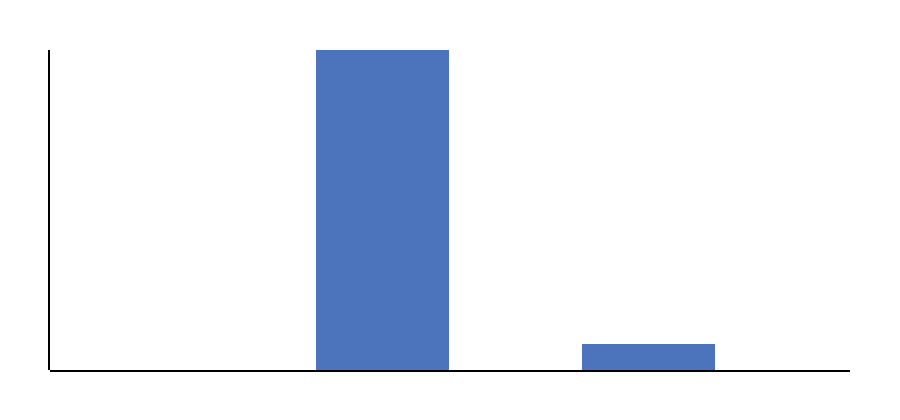
\includegraphics[width=0.72\linewidth]{../../experiments/results/latest/figures/gemini_real_eval.png}
\caption{Gemini-backed validation metrics for attack success, benign success, and tool blocking.}
\label{fig:gemini_validation}
\end{figure}
}{}

The Gemini-backed run completed with \texttt{gemini-2.5-flash-lite} on May 13, 2026. Across the 12-task stratified validation, SentinelAgent recorded 0.0\% attack success, 0.0\% measured secret leakage, 0.0\% unsafe tool invocation, 100.0\% benign success, and 3189.3 ms average end-to-end latency. One task was blocked at input screening before model planning; the remaining tasks exercised the real-model path. We treat this as useful engineering evidence that the wrapper can mediate a live planner. It is not the main ML result.

\section{Ablation Study}

\begin{table}[t]
\centering
\caption{Ablation Results}
\begin{tabular}{lrrrr}
\toprule
Profile & ASR & Leak & Benign & FPR \\
\midrule
no\_defense & 100.0\% [1.00,1.00] & 12.8\% & 100.0\% & 0.0\% \\
prompt\_only & 100.0\% [1.00,1.00] & 12.8\% & 100.0\% & 0.0\% \\
rules\_only & 24.0\% [0.20,0.28] & 3.2\% & 100.0\% & 0.0\% \\
ml\_only & 24.0\% [0.20,0.28] & 0.0\% & 100.0\% & 0.0\% \\
policy\_only & 43.2\% [0.38,0.47] & 0.0\% & 100.0\% & 40.0\% \\
full\_sentinelagent & 14.4\% [0.11,0.17] & 0.0\% & 100.0\% & 40.0\% \\
no\_retrieval\_screening & 19.2\% [0.16,0.22] & 0.0\% & 100.0\% & 40.0\% \\
no\_tool\_risk\_classifier & 50.4\% [0.46,0.55] & 0.0\% & 100.0\% & 0.0\% \\
no\_exfiltration\_detector & 14.4\% [0.11,0.17] & 0.0\% & 100.0\% & 40.0\% \\
no\_policy\_engine & 100.0\% [1.00,1.00] & 12.8\% & 100.0\% & 0.0\% \\
\bottomrule
\end{tabular}
\end{table}


The ablations show that the tool-risk component carries much of the protection for side-effecting tools. Removing the tool-risk classifier raises benchmark ASR from 14.4\% to 50.4\% and unsafe tool invocation from 15.6\% to 33.6\%. Removing retrieval screening also hurts: ASR rises to 19.2\%. Removing the exfiltration detector leaves the benchmark ASR unchanged in this generated run, but this should not be read as evidence that exfiltration detection is unnecessary. The adaptive set tells a different story.

\section{Adaptive Attack Analysis}

\begin{table}[t]
\centering
\caption{Adaptive Attack Results}
\begin{tabular}{lrrrr}
\toprule
Profile & ASR & Leak & Benign & FPR \\
\midrule
no\_defense & 100.0\% [1.00,1.00] & 100.0\% & 0.0\% & 0.0\% \\
prompt\_only & 100.0\% [1.00,1.00] & 100.0\% & 0.0\% & 0.0\% \\
rules\_only & 17.1\% [0.14,0.20] & 66.8\% & 0.0\% & 0.0\% \\
ml\_only & 0.0\% [0.00,0.00] & 0.0\% & 0.0\% & 0.0\% \\
policy\_only & 25.4\% [0.21,0.29] & 60.0\% & 0.0\% & 0.0\% \\
full\_sentinelagent & 16.4\% [0.13,0.20] & 50.9\% & 0.0\% & 0.0\% \\
no\_retrieval\_screening & 16.4\% [0.13,0.20] & 50.9\% & 0.0\% & 0.0\% \\
no\_tool\_risk\_classifier & 81.8\% [0.78,0.85] & 81.8\% & 0.0\% & 0.0\% \\
no\_exfiltration\_detector & 20.0\% [0.16,0.24] & 54.5\% & 0.0\% & 0.0\% \\
no\_policy\_engine & 100.0\% [1.00,1.00] & 100.0\% & 0.0\% & 0.0\% \\
\bottomrule
\end{tabular}
\end{table}


The adaptive suite is deliberately harder. It applies paraphrase, chunk splitting, markdown hiding, HTML comments, base64 and hex encoding, summarize-and-translate wrappers, tool-output injection, multi-turn escalation, and benign wrappers around malicious goals. Full SentinelAgent records 16.4\% ASR on adaptive attacks. More concerning, the adaptive leakage metric remains 50.9\% in the local simulator. That number reflects a weakness in the current output-control policy and evaluation mapping: many adaptive secret-exfiltration rows are monitored or routed through nonblocking paths rather than converted to response blocks.

This result is useful precisely because it is uncomfortable. It suggests that permission-aware policy reduces attack success but still needs stronger exfiltration controls, better encoded-payload handling, and more precise confirmation semantics before it should be evaluated with real side-effecting tools.

\section{Discussion}

Our results support three observations. First, the learned detector helps, but it needs enforcement context. A classifier score by itself does not know whether the agent is about to calculate a sum or send private content outside the system. Second, permissions matter. The same injected instruction has different consequences when attached to a calculator, private document search, external message sender, or database writer. Third, conservative policy can damage utility. SentinelAgent's current full profile blocks or interrupts benign high-risk tasks often enough to produce a 40.0\% false-positive rate in the benchmark.

The right interpretation is therefore not ``SentinelAgent solves prompt injection.'' It does not. The more careful claim is that risk-adaptive enforcement gives the system a place to make auditable, permission-sensitive decisions outside the model. That makes failures easier to inspect and policies easier to revise.

\section{Limitations}

The benchmark is generated, not collected from deployed enterprise agents. Generated benchmarks are useful for coverage and reproducibility, but they can overrepresent the patterns encoded by the generator. External corpora and red-team traces are needed before making broader claims.

The default agent mode is deterministic, and the primary aggregate results use the offline simulator. The Gemini-backed validation exercises a real planner, but only on 12 quota-limited tasks. Real LLM planners may behave differently under long-context pressure, social engineering, ambiguous tool-selection prompts, and larger tool menus. The LLM API path should therefore be read as an extension point for future work, not as the center of the present evaluation.

The ML detector is also limited. It is a compact n-gram Naive Bayes model trained from bundled fixtures, not a transformer model evaluated on a broad external corpus. Our results show that this lightweight model can support policy decisions in the generated benchmark, but stronger claims require outside datasets and adversarial traces.

The current policy treats user confirmation as an interruption and counts it as a false positive for benign tasks. That is conservative for security metrics, but human-centered studies are needed to decide when confirmation is acceptable friction.

The adaptive leakage results show a real gap. Encoded, translated, summarized, and multi-turn attacks need stronger final-response and tool-output controls than the current prototype applies.

\section{Related Work}

OWASP identifies prompt injection, sensitive information disclosure, and excessive agency as core LLM application risks \cite{owasp2025llm}. Greshake et al. demonstrate indirect prompt injection against LLM-integrated applications and motivate treating external content as untrusted \cite{greshake2023not}. Agent benchmarks such as InjecAgent and AgentDojo show why tool access changes the evaluation surface: an injected instruction can become a tool misuse, a privacy failure, or a persistence problem rather than only a bad answer \cite{zhan2024injecagent,debenedetti2024agentdojo}. Defense work on spotlighting, structured queries, and task-specific training explores ways to separate instructions from data or harden model behavior \cite{hines2024spotlighting,chen2024struq,piet2024jatmo}. NIST's AI Risk Management Framework emphasizes mapping, measuring, managing, and governing AI risks \cite{nist2023airmf}. SentinelAgent fits within that line of work as an implementation artifact that focuses on ML-assisted detection, tool permissions, and explicit enforcement boundaries.

Work on secure agent design also emphasizes least privilege, auditability, tool mediation, and constrained execution. SentinelAgent contributes a compact taxonomy and reproducible harness rather than a new model architecture. Its novelty is the direct coupling between prompt-injection risk and tool permission context.

\section{Conclusion}

SentinelAgent reframes prompt-injection defense for tool-using LLM agents as a risk-adaptive policy problem. The system models attack source, attack goal, target boundary, tool permissions, risk level, and enforcement action. It then applies deterministic gates around input, retrieved context, tool calls, tool outputs, and final responses.

The measured results are mixed in a productive way. Full SentinelAgent reduces benchmark ASR from 100.0\% to 14.4\% and removes measured benchmark secret leakage, while the supervised detector reaches 94.0\% accuracy on its held-out classifier split. At the same time, our policy introduces a 40.0\% false-positive rate and leaves substantial adaptive leakage. The small Gemini-backed validation records no successful attacks in 12 tasks, but that evidence is much narrower than the generated benchmark. The artifact is therefore best read as a research-grade prototype and reproducibility package, not a production security claim. Future work should expand the ML evaluation, add stronger output controls, tune confirmation policy, include external datasets, and test realistic side-effecting tools under strict sandboxing.

\appendix
\section{Artifact Appendix}

\subsection{Repository Structure}
\begin{lstlisting}
backend/sentinel_agent/research/taxonomy.py
backend/sentinel_agent/security/permissions.py
backend/sentinel_agent/security/policy_engine.py
backend/sentinel_agent/agent/llm_agent.py
backend/sentinel_agent/benchmark/generator.py
backend/sentinel_agent/benchmark/adaptive_attacks.py
experiments/run_evaluation.py
experiments/analyze_results.py
experiments/evaluate_classifier.py
experiments/datasets/
experiments/results/latest/
scripts/reproduce_paper.sh
scripts/reproduce_paper.ps1
Dockerfile.research
docker-compose.research.yml
ARTIFACT.md
\end{lstlisting}

\subsection{Reproduction Commands}
\begin{lstlisting}
cd sentinel-agent
scripts/reproduce_paper.sh
# optional real-model validation when Gemini keys are configured:
python experiments/run_llm_evaluation.py
\end{lstlisting}

On Windows PowerShell:
\begin{lstlisting}
cd sentinel-agent
.\scripts\reproduce_paper.ps1
# optional real-model validation when Gemini keys are configured:
python experiments\run_llm_evaluation.py
\end{lstlisting}

\subsection{Dataset Description}
The main benchmark is \path{experiments/datasets/sentinelagent_benchmark_v1.jsonl}. Each row includes a split, adversarial label, source, goal, boundary, tool context, required permissions, difficulty, payload, benign task, expected safe behavior, expected unsafe behavior, and labels. The adaptive set is test-only. The classifier dataset is separate and should not be used to train on the test split.

\subsection{Environment Details}
The evaluation runner writes \path{experiments/results/latest/environment.json} with timestamp, git commit hash when available, Python version, operating system, dependency versions, random seed, model backend, LLM provider, and model name. The corresponding manifest is \path{experiments/results/latest/reproducibility_manifest.json}. Real-model validation writes \path{experiments/results/latest/llm_gemini_metrics.json}, \path{experiments/results/latest/tables/gemini_results.tex}, and \path{experiments/results/latest/figures/gemini_real_eval.png}.

\begin{table}[t]
\centering
\caption{Latency Results}
\begin{tabular}{lrrrr}
\toprule
Profile & Mean ms & P50 ms & P95 ms & Throughput \\
\midrule
no\_defense & 1.73 & 1.68 & 2.19 & 578.3 \\
prompt\_only & 1.78 & 1.73 & 2.24 & 562.1 \\
rules\_only & 2.13 & 2.08 & 2.60 & 469.4 \\
ml\_only & 2.93 & 2.88 & 3.39 & 341.3 \\
policy\_only & 2.50 & 2.44 & 2.96 & 400.7 \\
full\_sentinelagent & 3.59 & 3.52 & 4.05 & 278.8 \\
no\_retrieval\_screening & 3.19 & 3.12 & 3.66 & 313.7 \\
no\_tool\_risk\_classifier & 2.98 & 2.92 & 3.45 & 335.1 \\
no\_exfiltration\_detector & 3.09 & 3.02 & 3.55 & 323.5 \\
no\_policy\_engine & 2.63 & 2.58 & 3.09 & 380.4 \\
\bottomrule
\end{tabular}
\end{table}


\bibliographystyle{plain}
\bibliography{../../report/references/references}

\end{document}
